98. а) $f(x)=\begin{cases} 4-|x+1|,\ x<2\\ x^2-6x+4,\ x\geqslant 2\end{cases}$
$$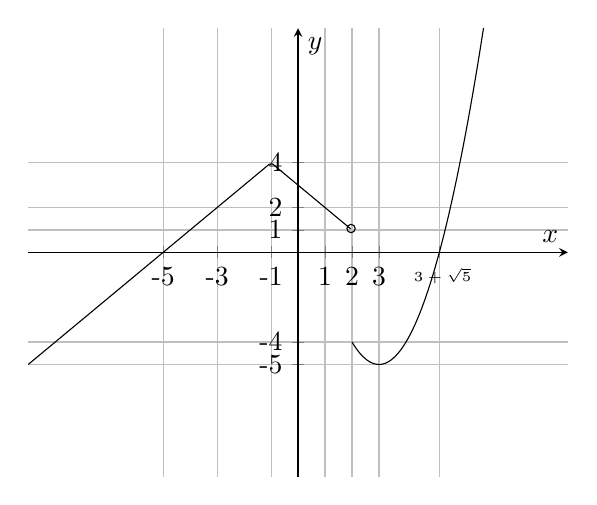
\begin{tikzpicture}[scale=1]
\tikzset{line03/.style={dashed,line width =0.9pt}}
\begin{axis}[
    axis lines = middle,
    grid=major,
    legend pos={south west},
    xlabel = {$x$},
    %xlabel style={below right},
    ylabel = {$y$},
    ymin=-10,
    ymax=10,
    xmin=-10,
    xmax=10,
    xtick={-5, -3, -1, 1, 2, 3, 5.236},
    xticklabels={-5, -3, -1, 1, 2, 3, \tiny{     $3+\sqrt{5}$}},
    ytick={4, 2, -4, 1, -5},
    yticklabels={$\text{4                    }$, 2, -4, 1, -5},        ]

	\addplot[domain=2:10, samples=100, color=black] {x*x-6*x+4};
	\addplot[domain=-10:1.95, samples=100, color=black] {4-abs(x+1)};

\end{axis}
\draw  (4.1,3.15) circle (1.5pt);
%\draw[line03] (3.11,0) -- (3.11,6);
%\draw[line03] (0,3.7) -- (6.5,3.7);
%\draw (3,5.7) node {\scriptsize $y$};
%\draw (7,2.5) node {\scriptsize $x$};
\end{tikzpicture}$$
б) По графику определим, что горизонатльная прямая $y=2a$ пересекает график функции $f(x)$ дважды в следующих случаях:
$2a=-5,\ 2a=4$ или $2a\in(-4;1],$ таким образом $a\in\left(-2;\cfrac{1}{2}
ight]\cup\left\{-\cfrac{5}{2};2
ight\}.$\\
